\documentclass[10pt,a4paper]{article}
% \documentclass[a4paper,
% 10pt,
% DIV 10]{scrartcl}

\usepackage[utf8x]{inputenc}
\usepackage[english]{babel}
\usepackage{amssymb}
\usepackage{amsmath}
\usepackage{amsmath}
\usepackage{url}
\usepackage{graphicx}
\usepackage{watermark}
\usepackage{xspace}
\usepackage{paralist}
\usepackage{xargs}
\usepackage{research}

\addtolength{\textheight}{-2cm}
\addtolength{\textwidth}{2cm}
\addtolength{\textheight}{4cm}
\addtolength{\oddsidemargin}{-12mm}


\pagestyle{empty}

\begin{document}
\watermark{\put(-95,-760){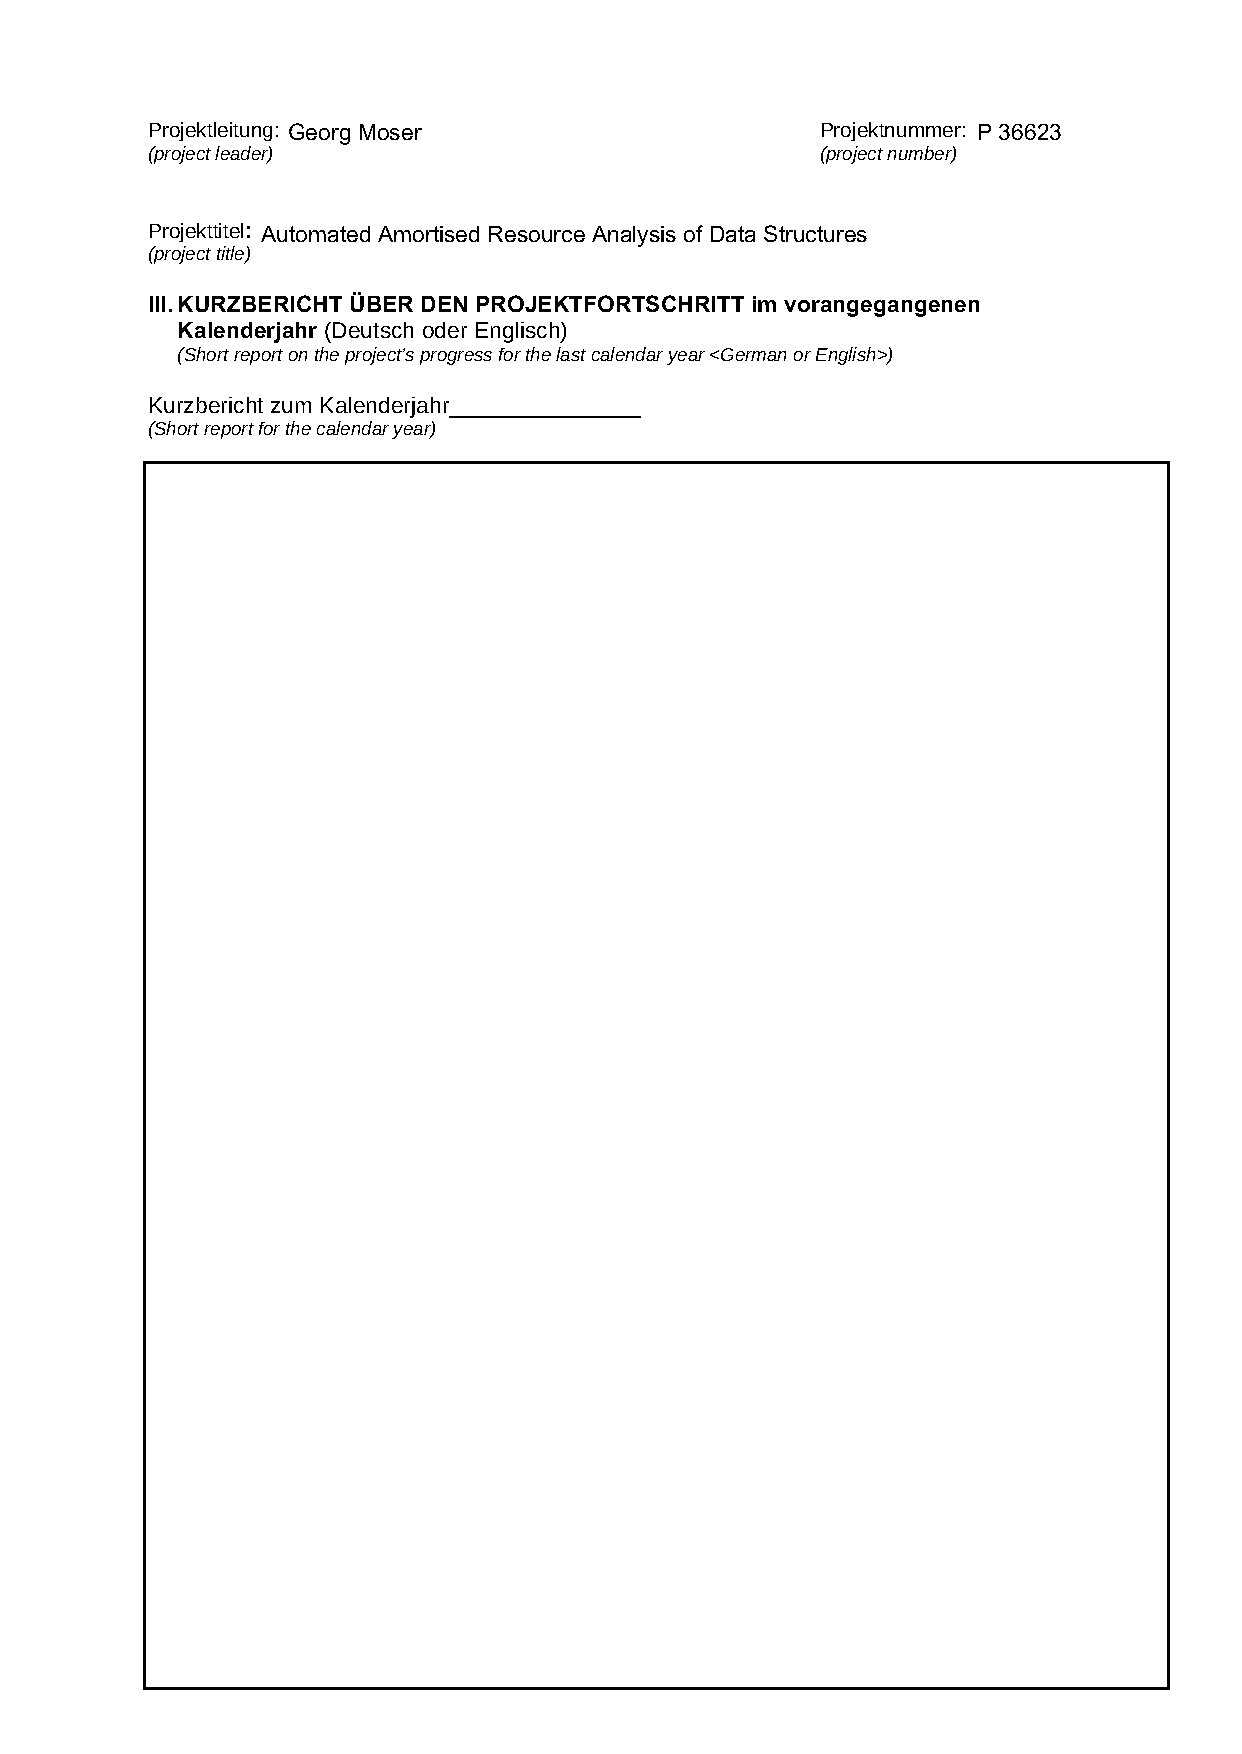
\includegraphics{template.pdf}}}

\vspace*{23mm}
\noindent\hspace{35ex}
2025

\vspace*{10mm}

\begin{center}
\large \normalsize Progress Report AUTOSARD 
\end{center}

After the project's initial phase, reported in last years' report, we have
one the one hand continued our work on the formalisation of data structures, but also worked mainly
towards Work Package~1 and~3.

With respect to the formalisation of data structures, we have been intensively working
on the formalisation of \emph{zip trees}, a probabilistic data structure recently developed
by Robert Tarjan, Caleb Levy and Stephen Timmel. Zip trees are isomorphic copies to
\emph{skip lists} introduced in 1990 by William Pugh.
%
In related work, we have provided a formalisation of skip lists based on so-called \emph{weakest-preconditions transformers}~\cite{AvanziniBGMV24}. Partly employing these ideas, but suitably adapted
to the---in our opinion---more elegant zip trees, we have been working on
a formalisation of the expected cost analysis of this data structure in Liquid Haskell, an interactive theorem prover, build on top of the functional
language \Haskell.

Further, we have investigated extensions of our ealier work during the pilot project within Armin Walch's master thesis~\cite{Walch:2025}. Here we have obtained a generalisation of the type system
underlying our prototype~\atlas. This theoretical investigations lead to the (fully) automated amortised
cost analyis of novel algorithms and formed the basis of a complete re-implementation of the prototype. The novel implementation, dubbed~\newatlas\ and performed in the programming language \Haskell, is more effective and more efficient at the same time.

Due to the novel implementation of the prototype from our pilot study, we have postponed our plans for journal version for pilot studies of AUTOSARD, that we want to complete
now, taking into account the more recent findings.
%
For further publication within the project, see~\cite{AvanziniMPP24}.

Finally, to improve dissemination of AUTOSARD's results, we hosted a workshop at the University Centre Obergurgl. Apart from project participants, we were joined by Bob Atkey, from the University of Strathclyde, UK; David Kahn, from Denison University, USA and our former colleage Lorenz Leutgeb now at MPI Saarbrücken. Among other talks, Atkey gave an inspiring tutorial on advanced type systems, Leutgeb presented a potentially interesting data structure for AUTOSARD, namely \emph{skew heaps} and Kahn spoke about the combinatorics of potential functions.

\bibliographystyle{plain}
\selectlanguage{english}
\small
\bibliography{references}

\end{document}
